\documentclass{standalone}
\usepackage{pgfplots}
\pgfplotsset{compat=1.13}
\usepackage{amsmath}

\begin{document}

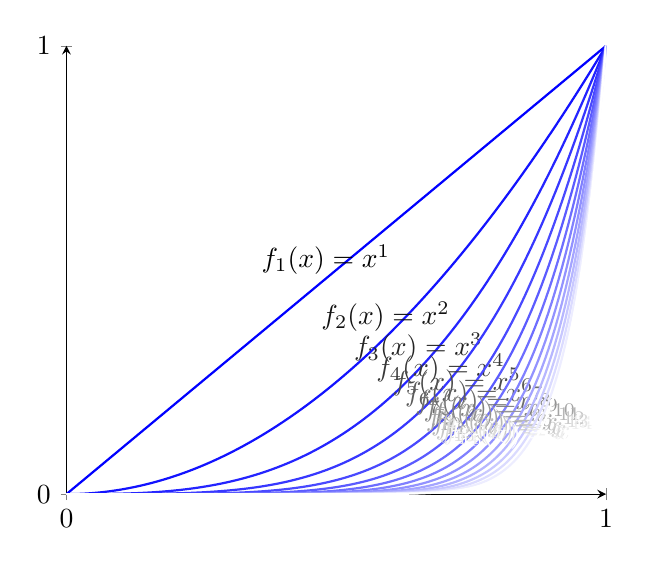
\begin{tikzpicture}
    \begin{axis}[
        axis y line = left,
        axis x line = bottom,
        xtick       = {0,1},
        xticklabels = {$0$,$1$},
        ytick       = {0,1},
        yticklabels = {$0$,$1$},
        samples     = 160,
        domain      = 0:1,
        xmin = 0, xmax = 1,
        ymin = 0, ymax = 1,
      ]
      \foreach[evaluate=\n as \redfrac using (\n-1)*100/(15-1)] \n in {1,...,15}{
          \edef\temp{
            \noexpand\addplot[white!\redfrac!blue, thick, mark=none, text = black] {x^\n} node[pos=0.5, above left] (mid) {};
            \noexpand\node[white!\redfrac!black] at (mid) {$f_{\n}(x) = x^{\n}$};
          }
          \temp
        }
    \end{axis}
  \end{tikzpicture}

\end{document}